%
% This work is licensed under a Creative Commons Attribution-ShareAlike 4.0 International License.
% http://creativecommons.org/licenses/by-sa/4.0/
%

% DO NOT COMPILE THIS FILE DIRECTLY!
% This is included by the other .tex files.


\begin{frame}
    
\includegraphics[scale=0.3]{images/logo-circl-Forensics.png}
    \begin{itemize}
        \item[]
        \item[]
        \item[] 4. Basic Malware Analysis
    \end{itemize}
\end{frame}


\begin{frame}[fragile]
  \frametitle{4.1 PE - Portable Execution format}
    \begin{itemize}
        \item Describe program files
        \item Contain:
        \begin{itemize}
            \item Meta data
            \item Instructions
            \item Text data
            \item Pictures and alike
        \end{itemize}
        \item Tell Windows how to load a program
        \item Provide resources to running program
        \item Provide resources like code signature
    \end{itemize}
  \begin{lstlisting}[basicstyle=\tiny]
      ---------------------------------------------
      |  1. DOS Header                            |
      |  2. PE Header                             |
      |  3. OPtional Header                       |
      |  4. Section Headers                       |
      |  5. .text Section (Program Code)          |
      |  6. .idata Section (Importd Libs)         |
      |  7. .rsrc Section (Strings, Images, ...)  |
      |  8. .reloc Section (Memory Translation)   |
      ---------------------------------------------
  \end{lstlisting}
\end{frame}


\begin{frame}[fragile]
  \frametitle{4.2 PE - Basic Analysis}
  \begin{lstlisting}[basicstyle=\tiny]
$ file 1.exe 
     malware/1.exe: PE32 executable (GUI) Intel 80386, for MS Windows


$ exiftool 1.exe

     File Name                       : 1.exe
     File Size                       : 300 kB
     .....
     Machine Type                    : Intel 386 or later, and compatibles
     Time Stamp                      : 2007:08:29 02:37:01+02:00
     PE Type                         : PE32
     Linker Version                  : 8.0
     Code Size                       : 57344
     Initialized Data Size           : 3940352
     Uninitialized Data Size         : 0
     Entry Point                     : 0x80c0
     OS Version                      : 4.0
     Subsystem                       : Windows GUI
     File OS                         : Windows NT 32-bit
     Object File Type                : Executable application
     .....
     Company Name                    : iWin Inc.
     File Description                : Furnishings
     Internal Name                   : Gem
     Legal Copyright                 : Dissipates (C) 2014
     Original File Name              : Glittering.exe
  \end{lstlisting}
\end{frame}


\begin{frame}[fragile]
  \frametitle{4.2 PE - Basic Analysis}
  \begin{lstlisting}[basicstyle=\tiny]
$ file Quotation.exe 
     Quotation.exe: PE32 executable (GUI) Intel 80386, for MS Windows


$ exiftool Quotation.exe
  
     ...
     Machine Type                    : Intel 386 or later, and compatibles
     Time Stamp                      : 2005:08:14 14:47:46+02:00
     PE Type                         : PE32
     Linker Version                  : 6.0
     Code Size                       : 647168
     Initialized Data Size           : 32768
     Uninitialized Data Size         : 0
     Entry Point                     : 0x15f4
     OS Version                      : 4.0
     ...  
     Character Set                   : Unicode
     Comments                        : Natcher
     Company Name                    : Glucosazone
     Legal Copyright                 : CRUSTER3
     Legal Trademarks                : Forearming
     Product Name                    : UNKLE
     File Version                    : 1.02.0009
     Product Version                 : 1.02.0009
     Internal Name                   : Aurous
     Original File Name              : Aurous.exe
  \end{lstlisting}
\end{frame}


\begin{frame}[fragile]
  \frametitle{4.2 PE - Basic Analysis}
  \begin{lstlisting}[basicstyle=\tiny]
$ python

     >>> import pefile
     >>> pe = pefile.PE("1.exe")
     >>> for section in pe.sections:
     ...      print(section.Name, section.VirtualAddress, 
                    section.Misc_VirtualSize, section.SizeOfRawData)
('.text\x00\x00\x00', 4096, 54028, 57344)
('.rdata\x00\x00', 61440, 4360, 8192)
('.data\x00\x00\x00', 69632, 3695044, 4096)
('.rsrc\x00\x00\x00', 3768320, 230456, 233472)



     >>> for entry in pe.DIRECTORY_ENTRY_IMPORT:
     ...     print(entry.dll)
     ...     for function in entry.imports:
     ...         print "\t",function.name

ADVAPI32.dll
        RegOpenKeyExA
        MapGenericMask
        AdjustTokenGroups
        SetSecurityDescriptorDacl
        GetSecurityDescriptorLength
        StartServiceA
        OpenServiceA
.....
  \end{lstlisting}
\end{frame}


\begin{frame}[fragile]
  \frametitle{4.2 PE - Basic Analysis}
  \begin{lstlisting}[basicstyle=\tiny]
$ strings 1.exe | less

     Microsoft Visual C++ Runtime Library
     ]]      ))
     ImageList_DragEnter
     ImageList_GetDragImage
     UninitializeFlatSB
     ImageList_SetOverlayImage
     ImageList_Merge
     COMCTL32.dll
     OLEAUT32.dll
     RegOpenKeyExA
     OpenServiceA
     StartServiceA
     GetSecurityDescriptorLength
     SetSecurityDescriptorDacl
     AdjustTokenGroups
     MapGenericMask
     ADVAPI32.dll
     .....


  mkdir images
$ wrestool -x 1.exe -o images/

  \end{lstlisting}
\end{frame}


\begin{frame}[fragile]
  \frametitle{4.2 PE - Basic Analysis}
  \begin{lstlisting}[basicstyle=\tiny]
$ strings Quotation.exe | less

     .....
     Damenization
     royle6
     nonexpedience
     incorporating1
     PEAS
     SIMOONS
     extramarginal
     ursula
     floricultural
     brainstorms
     NODDIES
     SCALOPUS9
     DEADHEADED
     lushai5
     elenchi7
     k40[
     VB5!6&*


  mkdir images
$ wrestool -x Quotation.exe -o images/

  \end{lstlisting}
\end{frame}


\begin{frame}[fragile]
  \frametitle{4.3 Enrich Online}
    \begin{itemize}
        \item Calculate hash values
  \begin{lstlisting}[basicstyle=\tiny]
$ md5sum 1.exe 
     a3bd288dec191caaed2057590e0dc34f

$ md5sum Quotation.*
e3f0a2033a78e307a71320217ef738bc  Quotation.exe
84617d594af613f77deb32927123f779  Quotation.zip

  \end{lstlisting}
        \item www.virustotal.com
        \begin{itemize}
	    \item[] $\to$ Live Demo
	    \item[] $\to$ Pro. Account
	    \item[] $\to$ Why not uploading office documents?
	    \item[]
        \end{itemize}
        \item MISP - Open Source Threat Intelligence Platform
        \begin{itemize}
		\item[] \url{https://www.misp-project.org/}
		\item[] \url{https://circl.lu/services/misp-malware-information-sharing-platform/}
	    \item[]
	    \item[] $\to$ Live Demo
	    \item[]
        \end{itemize}
    \end{itemize}
\end{frame}


\begin{frame}[fragile]
  \frametitle{4.3 Enrich Online}
    \begin{figure}
        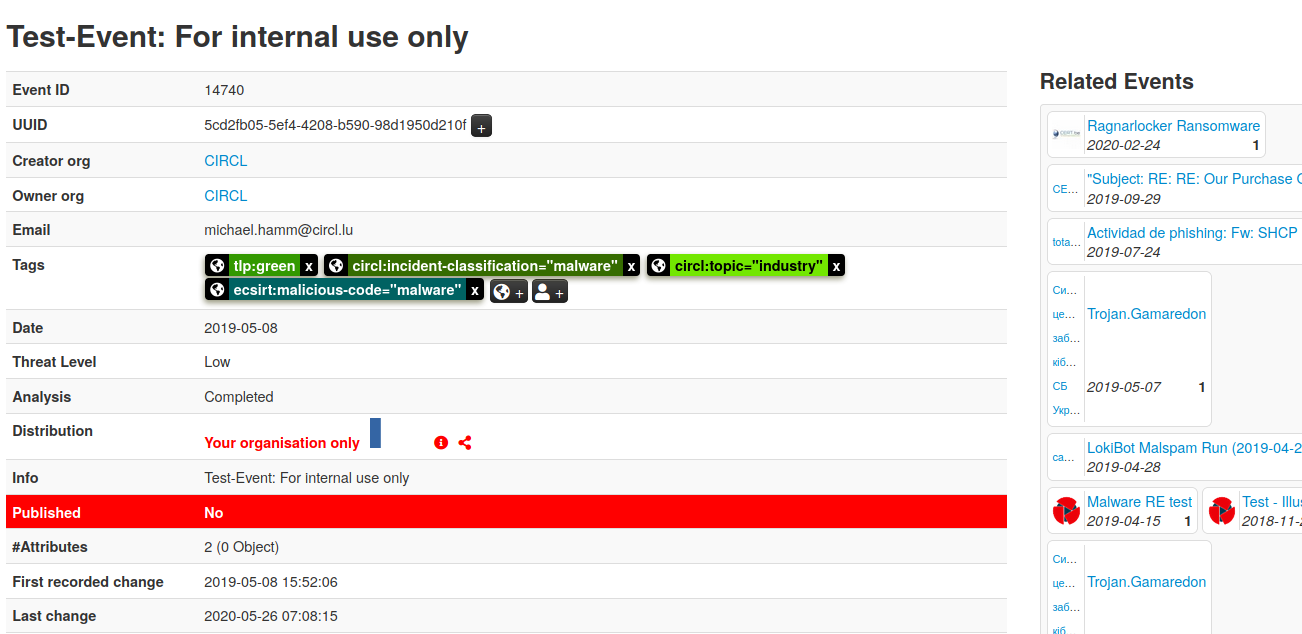
\includegraphics[scale=0.25]{images/misp_1.png}
        \captionsetup{labelformat=empty,labelsep=none}
        \transparent{0.7}%
        \caption[]{\tiny Event Overview: https://misppriv.circl.lu/}
    \end{figure}
\end{frame}


\begin{frame}[fragile]
  \frametitle{4.3 Enrich Online}
    \begin{figure}
        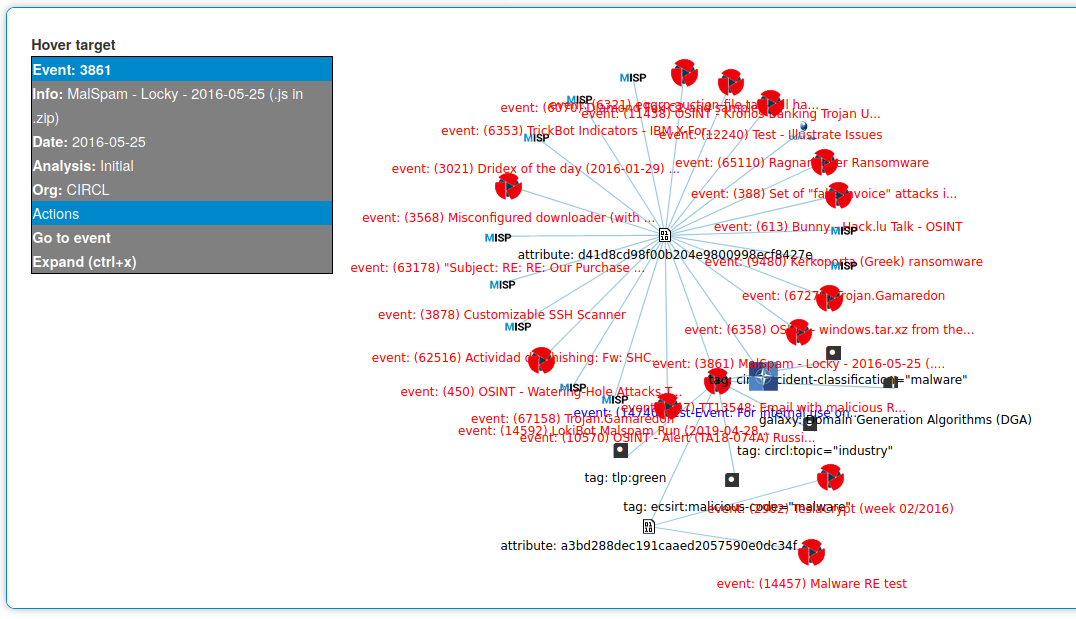
\includegraphics[scale=0.27]{images/misp_2.png}
        \captionsetup{labelformat=empty,labelsep=none}
        \transparent{0.7}%
        \caption[]{\tiny Correlation Graph: https://misppriv.circl.lu/}
    \end{figure}
\end{frame}


\begin{frame}[fragile]
  \frametitle{4.4 Static Analysis}
    \begin{itemize}
        \item Perfect disassembly $\to$ Unsolved problem
        \item Linear disassembly
        \begin{itemize}
            \item Identify the program code
            \item Decode the bytes
        \end{itemize}
        \item Linear disassembly limitations
        \begin{itemize}
            \item Don't know how instructions get decoded by CPU
            \item Could not counter fight obfuscation
        \end{itemize}
        \item Obfuscation techniques
        \begin{itemize}
            \item Packing
            \item Resource Obfuscation
            \item Anti-Disassembly
            \item Dynamic Data Download
        \end{itemize}
        \item Counter fight obfuscation
        \begin{itemize}
            \item Dynamic Analysis
            \item Run malware in isolated environment
        \end{itemize}
    \end{itemize}
\end{frame}


\begin{frame}[fragile]
  \frametitle{4.5 x86 Assembly: General-Purpose Registers}
    \begin{figure}
        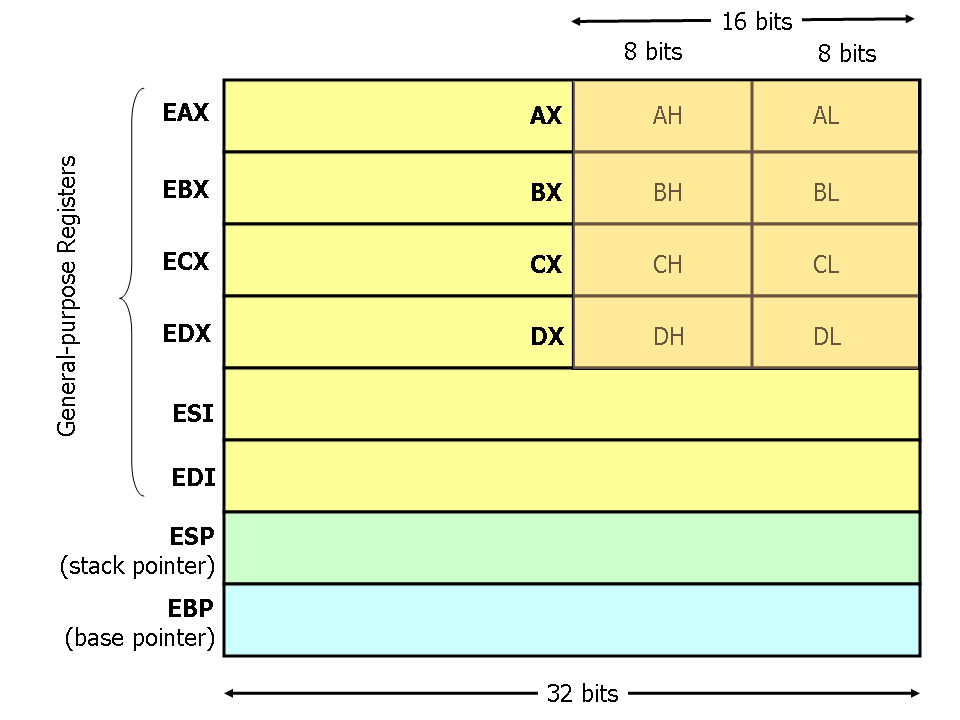
\includegraphics[scale=0.34]{images/x86-registers.png}
        \captionsetup{labelformat=empty,labelsep=none}
        \transparent{0.7}%
        \caption[]{\tiny https://www.cs.virginia.edu/~evans/cs216/guides/x86.html}
    \end{figure}
\end{frame}


\begin{frame}[fragile]
  \frametitle{4.5 x86 Assembly: Stack and Control Flow Registers}
    \begin{figure}
        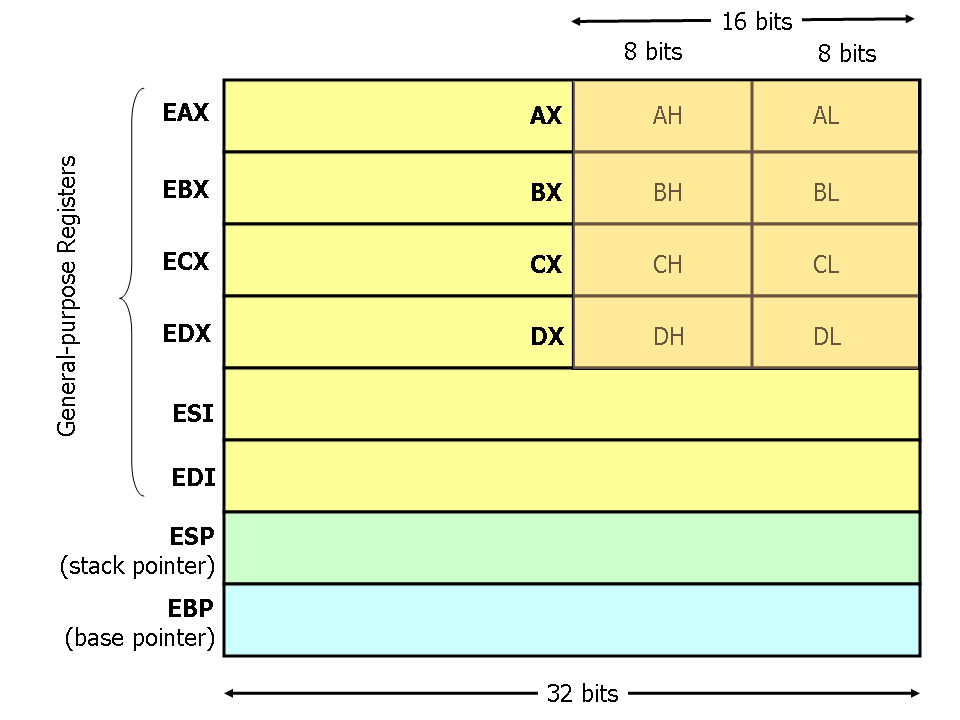
\includegraphics[scale=0.34]{images/x86-registers.png}
        \captionsetup{labelformat=empty,labelsep=none}
        \transparent{0.7}%
        \caption[]{\tiny https://www.cs.virginia.edu/~evans/cs216/guides/x86.html}
    \end{figure}
\end{frame}


\begin{frame}[fragile]
  \frametitle{4.5 x86 Assembly: Instructions}
  \begin{lstlisting}[basicstyle=\tiny]
Arithmetic:      add ebx, 100       Adds 100 to the value in EBX
                 sub ecx, 123       Substract 123 from the value in ECX
	         inc ah             Increments value in AH by 1
	         dec al             Decrements value in AL by 1

Data Movement:   mov eax, ebx       Move value in EBX into register EAX
                 mov eax, [0x4711]  Move value at memory 0x4711 intp EAX
		 mov eax, 1         Move the value 1 into register EAX
		 mov [0x4711], eax  Move value of EAX into memory 0x4711

Stack:           push 1             Increment ESP; Store 1 on top of stack
                 pop eax            Store highest value in EAX; Decrement ESP

Control Flow:    call [address]     1. Put EIP on top of the stack
                                    2. Put [address] into EIP
                 ret                1. Popped top of teh stack into EIP
		                    2. Resume execution
		 jmp 0x1234         Start executing progamm code at 0x1234
		 cmp eax, 100       1. Compares value in EAX with 100
		                    2. Based on result set EFLAGS register
		 jge 0x1234         1. Interpret EFLAGS register
		                    2. If 'greater' or 'equal' flag then jump
  \end{lstlisting}
\end{frame}


\begin{frame}[fragile]
  \frametitle{4.5 x86 Assembly: Control Flow Graphs}
  \begin{lstlisting}[basicstyle=\tiny]
start:             Symbol for address of next instruction
mov eax, 3         Initialize a counter of 3 into EAX

loop:              Symbol for address of next instruction
sub eax, 1         Substract 1 from value in EAX
cmp 0, eax         Compare value in EAX with 0; Set EFLAGS
jne $loop          IF EFLAGS 'not equal' jump to 'loop'

end:               Symbol for address of next instruction
mov eax, 12











.
  \end{lstlisting}
\end{frame}


\begin{frame}[fragile]
  \frametitle{4.5 x86 Assembly: Control Flow Graphs}
  \begin{lstlisting}[basicstyle=\tiny]
start:             Symbol for address of next instruction
mov eax, 3         Initialize a counter of 3 into EAX

loop:              Symbol for address of next instruction
sub eax, 1         Substract 1 from value in EAX
cmp 0, eax         Compare value in EAX with 0; Set EFLAGS
jne $loop          IF EFLAGS 'not equal' jump to 'loop'

end:               Symbol for address of next instruction
mov eax, 12


      -------------    ------>    -------------    ------>    ------------- 
     | start:      |      --->   | loop:       |             | end:        |
     | ----------- |     |       | ----------- |             | ----------- |
     |             |     |       |             |             |             |
     | mov eax, 3  |     |       | sub eax, 1  |             | mov eax, 12 |
     |             |     |       | cmp 0, eax  |             |             |
      -------------       ----   | jne $loop   |              -------------
			         |             | 
			          ------------- 
.
  \end{lstlisting}
\end{frame}


\begin{frame}[fragile]
  \frametitle{4.6 Dynamic Analysis}
    \begin{figure}
        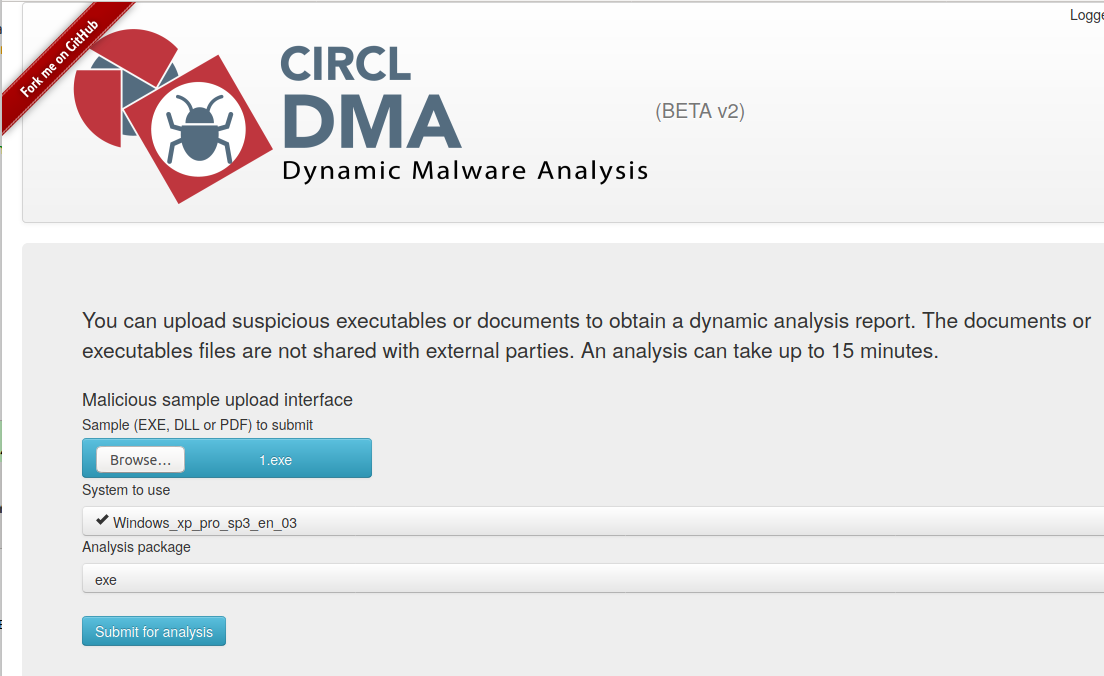
\includegraphics[scale=0.27]{images/dma_1.png}
        \captionsetup{labelformat=empty,labelsep=none}
        \transparent{0.7}%
        \caption[]{\tiny Upload a 1.exe: https://circl.lu/services/dynamic-malware-analysis/}
    \end{figure}
\end{frame}


\begin{frame}[fragile]
  \frametitle{4.6 Dynamic Analysis}
    \begin{figure}
        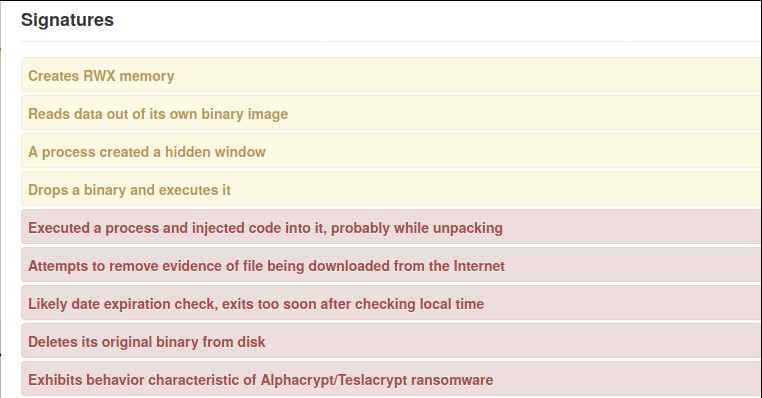
\includegraphics[scale=0.4]{images/dma_2a.png}
        \captionsetup{labelformat=empty,labelsep=none}
        \transparent{0.7}%
        \caption[]{\tiny Signatures and Screenshots: https://circl.lu/services/dynamic-malware-analysis/}
    \end{figure}
\end{frame}


\begin{frame}[fragile]
  \frametitle{4.6 Dynamic Analysis}
    \begin{figure}
        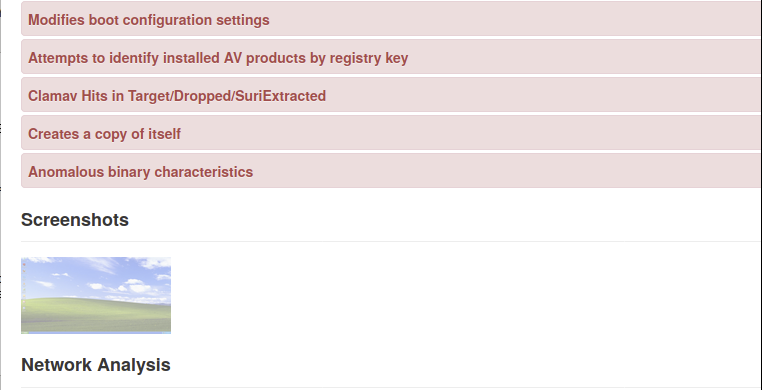
\includegraphics[scale=0.4]{images/dma_2b.png}
        \captionsetup{labelformat=empty,labelsep=none}
        \transparent{0.7}%
        \caption[]{\tiny Signatures and Screenshots: https://circl.lu/services/dynamic-malware-analysis/}
    \end{figure}
\end{frame}


\begin{frame}[fragile]
  \frametitle{4.6 Dynamic Analysis}
    \begin{figure}
        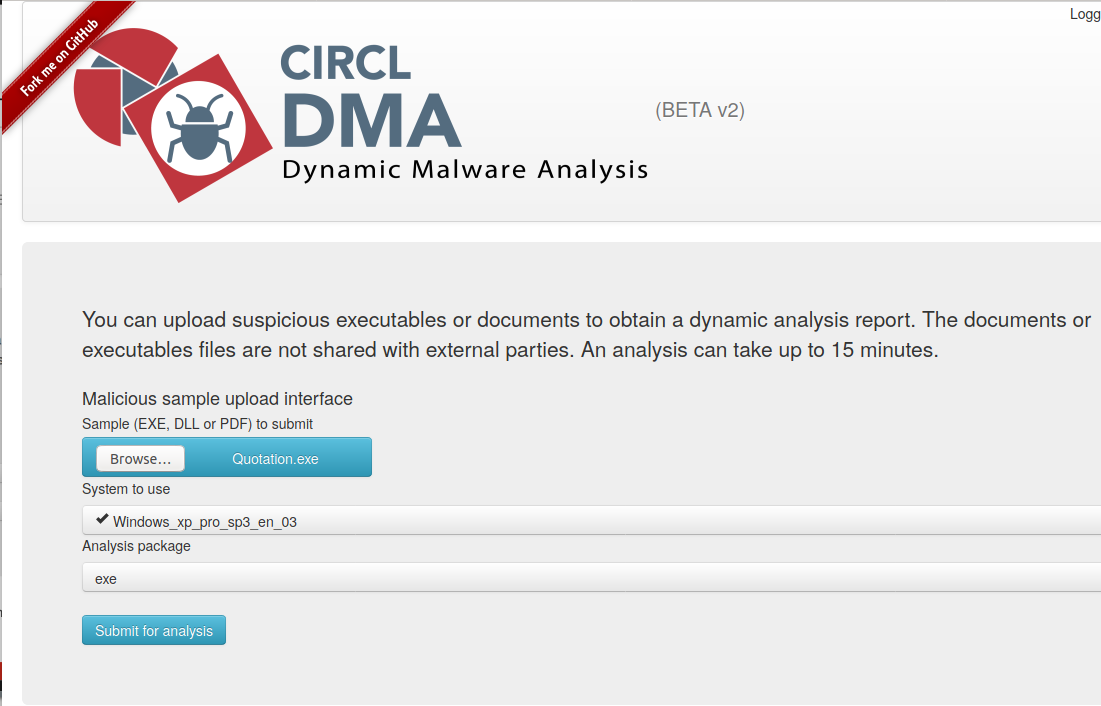
\includegraphics[scale=0.26]{images/dma_3.png}
        \captionsetup{labelformat=empty,labelsep=none}
        \transparent{0.7}%
        \caption[]{\tiny Upload a Quotation.exe: https://circl.lu/services/dynamic-malware-analysis/}
    \end{figure}
\end{frame}


\begin{frame}[fragile]
  \frametitle{4.6 Dynamic Analysis}
    \begin{figure}
        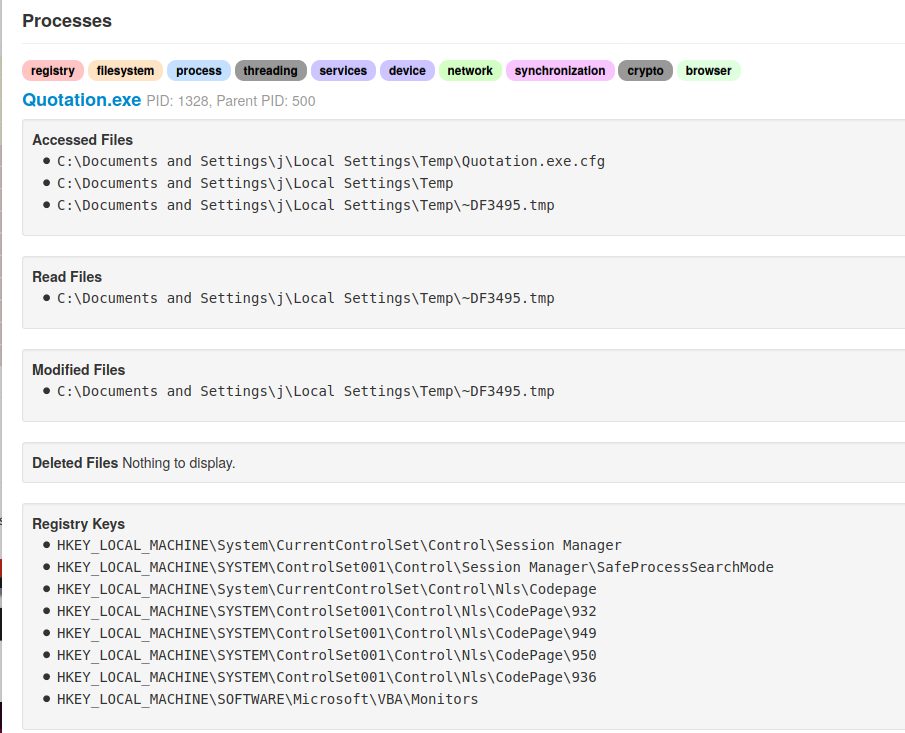
\includegraphics[scale=0.25]{images/dma_4.png}
        \captionsetup{labelformat=empty,labelsep=none}
        \transparent{0.7}%
        \caption[]{\tiny Access to Files and Registry: https://circl.lu/services/dynamic-malware-analysis/}
    \end{figure}
\end{frame}










